\section{Related Work}

Free variables in a 2D SBP-SAT scheme:
\begin{itemize} 
    \item{$N$: The problem size.}
    \item{$N_{0}$: the number of volume points in the $0\text{th}$ 
        dimension.}
    \item{$N_{1}$: the number of volume points in the $1\text{st}$ 
        dimension.}
\end{itemize}
With the constraint that 
$N_{0} \times N_{1} = N$. Resulting in the system
$A \kern 0.25em x \kern 0.125 em = \kern 0.125 em b$ 
where 
$\vert A \vert = N \times N$ \\
\noindent
The Hybridized scheme introduces additional free variables: 
\begin{itemize} 
    \item{$B$: The number of independent blocks.}
    \item{$K_{0}$: the number of flux interfaces in the $0\text{th}$ 
        direction.}
    \item{$K_{1}$: the number of flux interfaces in the $1\text{st}$ 
        dimension.}
\end{itemize}

With the constraint that $B = (K_{0} + 1) \times (K_{1} + 1)$. In this 
work we assume $K_{0} = K_{1}$ and use $K$ to refer to both $K_{0}$ and $K_{1}$, and write $B = (K + 1)^2$. \\ 

\noindent
The Hybridized scheme is given thusly: 

\begin{equation}
    \left[\begin{array}{cc}
        M & F \\
        F^T & D
    \end{array}\right] 
    \left(\begin{array}{c}
        u \\
        \lambda
    \end{array}\right) = 
    \left(\begin{array}{c}
        g \\
        g_\delta
    \end{array}\right)
\end{equation}


Expanding A...

\begin{equation}
    \left[\begin{array}{ccc | c}
        m_0 & & & f_0 \\
        & \ddots & & \vdots \\
        & & m_{B-1} & f_{B-1} \\ \hline
        f^T_0 & & f^T_{B-1} & D
    \end{array}\right] 
\end{equation}

In plain language, The $F$ and $F^T$ contain boundary and interface data 
for each block. 

\begin{equation}
(D - F^T M^{-1} F) \lambda = g_\delta - F^T M^{-1} g
\end{equation}

\begin{equation}
 \lambda = \frac{g_\delta - {\color{blue}F^T} \times \text{solve}({\color{blue}M}, {\color{blue}g})}{D - {\color{blue}F^T} \times {\color{red}\text{solve}}({\color{blue}M}, {\color{blue}F})}
\end{equation}

\begin{equation}
    \lambda = (g_{\delta} - \textbf{F}^{\intercal} \textbf{M}^{-1} g)^{-1} (\textbf{D} - \textbf{F}^{\intercal} \textbf{M}^{-1} \textbf{F})
\end{equation}

\begin{lstlisting}
g := b + <boundary data>
lambda_A := g_del - F × solve(M, g)
MF := similar(F)
for col in columns(F)
    MF[:, col] := solve(M, F[:, col])
lambda_b := D - FT × MF
lambda := solve(lambda, lambda)
u := solve(M, g_bar - F × lambda)
\end{lstlisting}



To simplify computation of the 2D problem we observe that the matrices $\textbf{F}$ and $\textbf{F}^\textbf{F}$ are assembled of simpler sub-matrices $\textbf{F}_{4}$, $\textbf{F}_3$, $\textbf{F}_1$, $\textbf{F}_{2}$ encoding boundary coefficients. Given a $3 \times 3$ block problem with a volume ordering of 

\subsection{An example.}

\noindent 
Here we solve Poisson's equation in 2D on a square volume with Dirichlet boundary conditions on faces 0 and 1, and Neumann boundary conditions on global faces 2 and 3. 

\begin{center}
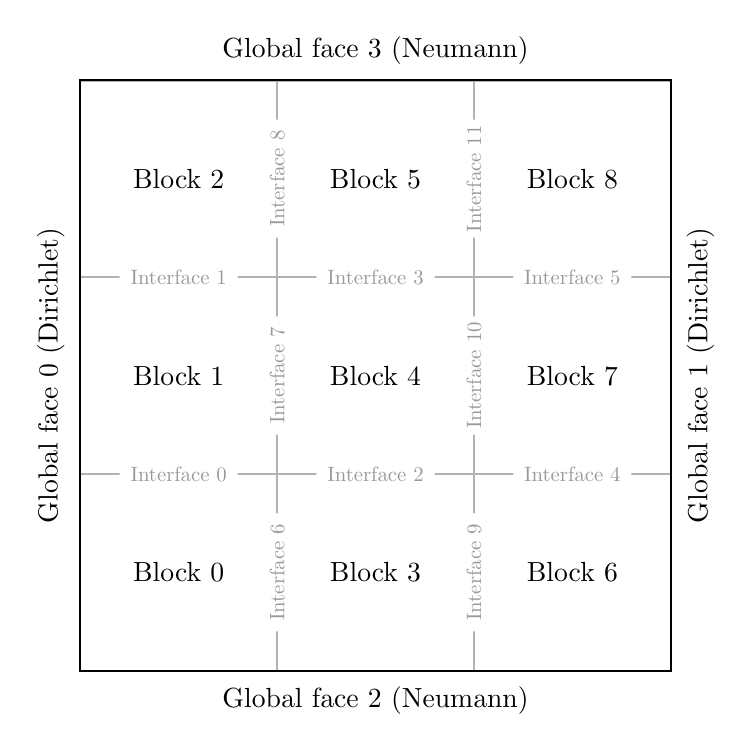
\begin{tikzpicture}[scale=2.5]
\draw[step=1cm,black!30,line width=0.3mm] (0, 0) grid (3, 3);
\draw[line width=0.3mm] (0, 0) rectangle (3, 3);

\fill[white] (0.5cm, 1cm) circle (0.3cm);
\node[color=black!40, scale=0.75] at (0.5cm, 1cm) {Interface 0};
\fill[white] (0.5cm, 2cm) circle (0.3cm);
\node[color=black!40, scale=0.75] at (0.5cm, 2cm) {Interface 1};
\fill[white] (1.5cm, 1cm) circle (0.3cm);
\node[color=black!40, scale=0.75] at (1.5cm, 1cm) {Interface 2};
\fill[white] (1.5cm, 2cm) circle (0.3cm);
\node[color=black!40, scale=0.75] at (1.5cm, 2cm) {Interface 3};
\fill[white] (2.5cm, 1cm) circle (0.3cm);
\node[color=black!40, scale=0.75] at (2.5cm, 1cm) {Interface 4};
\fill[white] (2.5cm, 2cm) circle (0.3cm);
\node[color=black!40, scale=0.75] at (2.5cm, 2cm) {Interface 5};

\fill[white](1cm, 0.5cm) circle (0.3cm);
\node[color=black!40, rotate=90, scale=0.75] at (1cm, 0.5cm) {Interface 6};
\fill[white] (1cm, 1.5cm) circle (0.3cm);
\node[color=black!40, rotate=90, scale=0.75] at (1cm, 1.5cm) {Interface 7};
\fill[white] (1cm, 2.5cm) circle (0.3cm);
\node[color=black!40, rotate=90, scale=0.75] at (1cm, 2.5cm) {Interface 8};
\fill[white] (2cm, 0.5cm) circle (0.3cm);
\node[color=black!40, rotate=90, scale=0.75] at (2cm, 0.5cm) {Interface 9};
\fill[white] (2cm, 1.5cm) circle (0.3cm);
\node[color=black!40, rotate=90, scale=0.75] at(2cm, 1.5cm) {Interface 10};
\fill[white] (2cm, 2.5cm) circle (0.3cm);
\node[color=black!40, rotate=90, scale=0.75] at (2cm, 2.5cm) {Interface 11};


\draw (0.5cm, 0.5cm) -- (0.5cm, 0.5cm) node[anchor=center] {Block 0};
\draw (0.5cm, 1.5cm) -- (0.5cm, 1.5cm) node[anchor=center] {Block 1};
\draw (0.5cm, 2.5cm) -- (0.5cm, 2.5cm) node[anchor=center] {Block 2};
\draw (1.5cm, 0.5cm) -- (1.5cm, 0.5cm) node[anchor=center] {Block 3};
\draw (1.5cm, 1.5cm) -- (1.5cm, 1.5cm) node[anchor=center] {Block 4};
\draw (1.5cm, 2.5cm) -- (1.5cm, 2.5cm) node[anchor=center] {Block 5};
\draw (2.5cm, 0.5cm) -- (2.5cm, 0.5cm) node[anchor=center] {Block 6};
\draw (2.5cm, 1.5cm) -- (2.5cm, 1.5cm) node[anchor=center] {Block 7};
\draw (2.5cm, 2.5cm) -- (2.5cm, 2.5cm) node[anchor=center] {Block 8};


\node[rotate=90] at (-0.15cm, 1.5cm) {Global face 0 (Dirichlet)};
\node[rotate=90] at (3.15cm, 1.5cm) {Global face 1 (Dirichlet)};
\node at (1.5cm, -0.15cm) {Global face 2 (Neumann)};
\node at (1.5cm, 3.15cm)  {Global face 3 (Neumann)};
\end{tikzpicture}
\end{center}

\noindent
A matrix of block-to-block mappings encodes which blocks a given interface interacts with:

\begin{equation}
    \begin{array}{c}
        \textit{\color{gray} Block index }  \\ 
        {\color{gray}
        \begin{array}{*9{C{0.5em}}c}
            {0}&{1}&{2}&{3}&{4}&{5}&{6}&{7}&{8}&{\hspace{-0.5em}}\\
        \end{array}} \\
        \textbf{B} = \left[\begin{array}{*9{C{0.5em}}}
            {·}&{0}&{·}&{6}&{·}&{·}&{·}&{ ·}&{ ·}\\
            {·}&{·}&{1}&{·}&{7}&{·}&{·}&{ ·}&{ ·}\\
            {·}&{·}&{·}&{·}&{·}&{8}&{·}&{ ·}&{ ·}\\
            {·}&{·}&{·}&{·}&{2}&{·}&{9}&{ ·}&{ ·}\\
            {·}&{·}&{·}&{·}&{·}&{3}&{·}&{10}&{ ·}\\
            {·}&{·}&{·}&{·}&{·}&{·}&{·}&{ ·}&{11}\\
            {·}&{·}&{·}&{·}&{·}&{·}&{·}&{ 4}&{ ·}\\
            {·}&{·}&{·}&{·}&{·}&{·}&{·}&{ ·}&{ 5}\\
            {·}&{·}&{·}&{·}&{·}&{·}&{·}&{ ·}&{ ·}\\
        \end{array}\right] {\color{gray}
    \begin{array}{C{0.5em}}
        0 \\ 1 \\ 2 \\ 3 \\ 4 \\ 5 \\ 6 \\ 7 \\ 8
    \end{array}{\rotatebox[origin=c]{90}{\textit{Block index}}}} 
    \end{array}. \\
\end{equation}
\noindent
Notably here, the first off-diagonal contains all boundaries parallel to global faces 2 and 3, while the second off diagonal contains all boundaries parallel to global faces 0 and 1. 

From this we derive $\textbf{F}$ and $\textbf{F}^\intercal$ given in terms of boundary coefficient matrices
\begin{equation}
    \begin{array}{c}
        {\color{gray} \hspace{-1em} \textit{Interface index}} \\
        {\color{gray}
        \begin{array}{C{1em}C{1em}C{1em}C{1em}C{1em}C{1em}C{1em}C{1em}C{1em}C{1em}C{1em}C{1em}C{1em}C{2em}}
        {}&{0}&{1}&{2}&{3}&{4}&{5}&{6}&{7}&{8}&{9}&{10}&{11}&{}\\
        \end{array}} \\
        \textbf{F} = \left[\begin{array}{cccccccccccc}
        \textbf{F}_3&{·}&{·}&{·}&{·}&{·}&\textbf{F}_1&{·}&{·}&{·}&{·}&{·}\\
        \textbf{F}_2&\textbf{F}_3&{·}&{·}&{·}&{·}&{·}&\textbf{F}_1&{·}&{·}&{·}&{·}\\
        {·}&\textbf{F}_2&{·}&{·}&{·}&{·}&{·}&{·}&\textbf{F}_1&{·}&{·}&{·}\\
        {·}&{·}&\textbf{F}_3&{·}&{·}&{·}&\textbf{F}_0&{·}&{·}&\textbf{F}_1&{·}&{·}\\
        {·}&{·}&\textbf{F}_2&\textbf{F}_3&{·}&{·}&{·}&\textbf{F}_0&{·}&{·}&\textbf{F}_1&{·}\\
        {·}&{·}&{·}&\textbf{F}_2&{·}&{·}&{·}&{·}&\textbf{F}_0&{·}&{·}&\textbf{F}_1\\
        {·}&{·}&{·}&{·}&\textbf{F}_3&{·}&{·}&{·}&{·}&\textbf{F}_0&{·}&{·}\\
        {·}&{·}&{·}&{·}&\textbf{F}_2&\textbf{F}_3&{·}&{·}&{·}&{·}&\textbf{F}_0&{·}\\
        {·}&{·}&{·}&{·}&{·}&\textbf{F}_2&{·}&{·}&{·}&{·}&{·}&\textbf{F}_0\\
        
        \end{array}\right] {\color{gray}
        \begin{array}{C{1em}}
         0 \\ 1 \\ 2 \\ 3 \\ 4 \\ 5 \\ 6 \\ 7 \\ 8
        \end{array}{\rotatebox[origin=c]{90}{\textit{Block index}}}} \\
    \end{array}
\end{equation}

\begin{equation}
    \begin{array}{c}
        {\color{gray} \hspace{-1em} \textit{Block index}} \\
        {\color{gray}
        \begin{array}{C{0em}C{1em}C{1em}C{1em}C{1em}C{1em}C{1em}C{1em}C{1em}C{1em}C{1em}}
        {}&{0}&{1}&{2}&{3}&{4}&{5}&{6}&{7}&{8}&{}\\
        \end{array}} \\
        \small
        \textbf{F}^{\intercal} = \left[\begin{array}{ccccccccc}
        \textbf{F}^{\intercal}_3&\textbf{F}^{\intercal}_2&{·}&{·}&{·}&{·}&{·}&{·}&{·}\\
        {·}&\textbf{F}^{\intercal}_3&\textbf{F}^{\intercal}_2&{·}&{·}&{·}&{·}&{·}&{·}\\
        {·}&{·}&{·}&\textbf{F}^{\intercal}_3&\textbf{F}^{\intercal}_2&{·}&{·}&{·}&{·}\\
        {·}&{·}&{·}&{·}&\textbf{F}^{\intercal}_3&\textbf{F}^{\intercal}_2&{·}&{·}&{·}\\
        {·}&{·}&{·}&{·}&{·}&{·}&\textbf{F}^{\intercal}_3&\textbf{F}^{\intercal}_2&{·}\\
        {·}&{·}&{·}&{·}&{·}&{·}&{·}&\textbf{F}^{\intercal}_3&\textbf{F}^{\intercal}_2\\
        \textbf{F}^{\intercal}_1&{·}&{·}&\textbf{F}^{\intercal}_0&{·}&{·}&{·}&{·}&{·}\\
        {·}&\textbf{F}^{\intercal}_1&{·}&{·}&\textbf{F}^{\intercal}_0&{·}&{·}&{·}&{·}\\
        {·}&{·}&\textbf{F}^{\intercal}_1&{·}&{·}&\textbf{F}^{\intercal}_0&{·}&{·}&{·}\\
        {·}&{·}&{·}&\textbf{F}^{\intercal}_1&{·}&{·}&\textbf{F}^{\intercal}_0&{·}&{·}\\
        {·}&{·}&{·}&{·}&\textbf{F}^{\intercal}_1&{·}&{·}&\textbf{F}^{\intercal}_0&{·}\\
        {·}&{·}&{·}&{·}&{·}&\textbf{F}^{\intercal}_1&{·}&{·}&\textbf{F}^{\intercal}_0\\
        \end{array}\right] {\color{gray}
        \begin{array}{r}
         0 \\ 1 \\ 2 \\ 3 \\ 4 \\ 5 \\ 6 \\ 7 \\ 8 \\ 9 \\ 10 \\ 11
        \end{array}{\rotatebox[origin=c]{90}{\textit{Interface index}}}} \\
    \end{array}
\end{equation}

\noindent
shaped by the number of blocks and and the number of interfaces and encoded by the indices of entries in $\textbf{B}$. \emph{E.g.}, block 1 and block 3 share an east-west interface, notated by $\mathcal{B}_{[1, 3]} = \textbf{F}_1$ and $\mathcal{S}_{[3, 1]} = \textbf{F}_{2}$, in row 1 of $\textbf{F}_{\mathcal{S}}$ we place a $\textbf{F}_1$ and row 3 of $\textbf{F}_{\mathcal{S}}$ we place a $\textbf{F}_{2}$ in the same column; here column (interface) ordering is critically important, as long as it is symbolically consistent between $\textbf{F}_{\mathcal{S}}$ and $\textbf{F}_{\mathcal{S}}^{\textbf{F}}$.\footnote{For later operations there may exist more optimal interface orderings.} Importantly $\textbf{F}_{\mathcal{S}}^{\textbf{F}}$ is indeed the transpose of the $\textbf{F}_{\mathcal{S}}$, but requiring the transpose of all boundary coefficient matrices for $(\textbf{F})^{\textbf{F}} \equiv \textbf{F}^{\textbf{F}}$ to hold.

With this we determine a minimally set of necessary computations between blocks $\textbf{m} \in \textbf{M}$ and the set of boundary coefficient matrices, $\{\textbf{F}_{4}$, $\textbf{F}_3$, $\textbf{F}_1$, $\textbf{F}_{2}\}$ to compute $\text{solve}(\textbf{M}, \textbf{F})$. \emph{E.g.}, block 3 shares a $\textbf{F}_{2}$, $\textbf{F}_{4}$, and $\textbf{F}_1$ interface, requiring solutions to the systems
\begin{itemize}
    \item $\textbf{m}_3 x_{(3,\textbf{F}_{2})} = \textbf{F}_{2}$
    \item $\textbf{m}_3 x_{(3,\textbf{F}_{4})} = \textbf{F}_{4}$
    \item $\textbf{m}_3 x_{(3,\textbf{F}_1)} = \textbf{F}_1$
\end{itemize}
\noindent 
where $x_{(3,\textbf{F}_{2})}$, $x_{(3,\textbf{F}_{4})}$, $x_{(3,\textbf{F}_1)}$ are unknown; however as several blocks in $\textbf{M}$ are equivalent, the minimal set of necessary computations will be significantly smaller than $|\textbf{M}| \times \text{nnz}(\textbf{F}_{\mathcal{S}})$. This is given in an expanded form as 

%\begin{equation}
%    \textbf{x}^{*}_{\mathcal{S}}= \left[\begin{array}{cccccccccccc}
    
%    \textbf{x}_{[0, \textbf{F}_{4})}   & \cdot      & \textbf{x}_{[0, \textbf{F}_1]}  & \cdot       & \cdot      & \cdot       & \cdot      & \cdot       & \cdot       & \cdot      & \cdot       & \cdot \\     
%    \textbf{x}_{[1, \textbf{F}_3]} & \textbf{x}_{[1, \textbf{F}_{4}]}   & \cdot       & \textbf{x}_{[1, \textbf{F}_1]}  & \cdot      & \cdot       & \cdot      & \cdot       & \cdot       & \cdot      & \cdot       & \cdot \\     
%    \cdot      & \textbf{x}_{[2, \textbf{F}_3]} & \cdot       & \cdot       & \cdot      & \textbf{x}_{[2, \textbf{F}_1]}  & \cdot      & \cdot       & \cdot       & \cdot      & \cdot       & \cdot \\     
%    \cdot      & \cdot      & \textbf{x}_{[3, \textbf{F}_{2}]} & \cdot       & \textbf{x}_{[3, \textbf{F}_{4}]}   & \cdot       & \cdot      & \textbf{x}_{[3, \textbf{F}_1]}  & \cdot       & \cdot      & \cdot       & \cdot \\     
%    \cdot      & \cdot      & \cdot       & \textbf{x}_{[4, \textbf{F}_{2}]} & \textbf{x}_{[4, \textbf{F}_3]} & \cdot       & \textbf{x}_{[4, \textbf{F}_{4}]}   & \cdot       & \textbf{x}_{[4, \textbf{F}_1]} & \cdot      & \cdot       & \cdot \\     
%    \cdot      & \cdot      & \cdot       & \cdot       & \cdot      & \textbf{x}_{[5, \textbf{F}_{2}]} & \textbf{x}_{[5, \textbf{F}_3]} & \cdot       & \cdot       & \cdot      & \textbf{x}_{[5,\textbf{F}_1]}  & \cdot \\     
%    \cdot      & \cdot      & \cdot       & \cdot       & \cdot      & \cdot       & \cdot      & \textbf{x}_{[6, \textbf{F}_{2}]} & \cdot       & \textbf{x}_{[6, \textbf{F}_{4}]}   & \cdot       & \cdot \\     
%    \cdot      & \cdot      & \cdot       & \cdot       & \cdot      & \cdot       & \cdot      & \cdot       & \textbf{x}_{[7, \textbf{F}_{2}]} & \textbf{x}_{[7, \textbf{F}_3]} & \cdot       & \textbf{x}_{[7, \textbf{F}_{4}]} \\     
%    \cdot      & \cdot      & \cdot       & \cdot       & \cdot      & \cdot       & \cdot      & \cdot       & \cdot       & \cdot      & \textbf{x}_{[8, \textbf{F}_{2}]} & \textbf{x}_{[8, \textbf{F}_3]} \\     

%    \end{array}\right] {\color{gray}
%    \begin{array}{c}
%     0 \\ 1 \\ 2 \\ 3 \\ 4 \\ 5 \\ 6 \\ 7 \\ 8
%    \end{array}{\rotatebox[origin=c]{90}{\textit{Block index}}}} 
%\end{equation}

\noindent and stores the intermediary component of computing $\textbf{D} - \textbf{F}^\textbf{F} \times \text{solve}(\textbf{MF}) \equiv \textbf{D} - \textbf{F}^\textbf{F} \times \textbf{x}^{*}$.


\noindent

\subsection{Solving the matrix-matrix system}

\begin{itemize}
    \item \textbf{Outright matrix-by-column} 
    \begin{lstlisting} 
    M = mat{}
    F = [vec{}, ..., vec{}]
    X = [vec{}, ..., vec{}]

    for col in n_cols
        X[i] = solve(M, F[col])
    end\end{lstlisting}
    \item \textbf{Matrix block-by-column} 
    \begin{lstlisting} 
    M = [mat{}, ..., mat{}]
    F = [list{vec{}}, ..., list{vec{}}]
    X = [list{vec{}}, ..., list{vec{}}]

    for block in n_blocks
        for col in n_cols
            X[block][col] = solve(M[block], F[i][col])
        end
    end\end{lstlisting}

    \item \textbf{Factored solve} 
    \begin{lstlisting} 
    M_set = [mat{}, mat{}, mat{}]
    F_set = [list{vec{}}, list{vec{}}, list{vec{}}, list{vec{}}]
    solves = [list{vec{}}, ... , list{vec{}}]
    X = [list{vec{}}, ... , list{vec{}}]

    // Compute all factored solves 
    for block in length(M_set) 
        for factor in length(F_set)
            for col in n_cols
                solve[block * factor + factor][col] = solve(M_set[block], F_set[factor][col])
            end
        end
    end

    unique = [(i_0, x_0, y_0), ... , (i_k, x_n, y_n)]

    // Write from computed factors 

    for i, x, y in unique 
        for col in n_cols 
            X[x][y][col] = solve[i][col]
        end
    end
    end\end{lstlisting}

\end{itemize}
